\section{Recorded results and remaining gaps}
\label{sec:v2results}
All numerical quantities in this section are generated from validated v2
evidence. The older synthetic results are retained against their original
revision in the appendices. A fresh run of the v1 pipeline checks compatibility;
it is not substituted for either the v2 protocol evidence or an adversarial
language-model evaluation.

\begin{table}[t]\centering\small\begin{tabularx}{\columnwidth}{@{}Lr@{}}\toprule
Recorded check & Result\\\midrule
Application core obligations & 17 verified\\
Sequential fault histories & 24 passed\\
Concurrent race repetitions & 18 passed\\
Abstract omission sets with witnesses & 55/55\\
Native benchmark utility positives & 12/12\\
Model campaigns & Unrun\\
\bottomrule\end{tabularx}\caption{Evidence types remain distinct. Abstract mutation witnesses and native scripted controls are not adversarial model measurements.}\label{tab:v2summary}\end{table}
\begin{table}[t]\centering\small\begin{tabularx}{\columnwidth}{@{}Lrr@{}}\toprule
CPU controller & Safe/useful & Runs\\\midrule
No enforcement & 3/18 & 18\\
Stateless per-call & 3/18 & 18\\
Durable, no fence & 18/18 & 18\\
Complete & 18/18 & 18\\
Learned, same checkpoint & Unrun & 0\\
\bottomrule\end{tabularx}\caption{Sequential scripted shared-budget controls over all six actor populations, with equal permissions. These descriptive outcomes do not support model noninferiority.}\label{tab:v2controllers}\end{table}
The delayed-completion control measured a fence acknowledgment delay of 578.29 ms with 8 units unavailable at acknowledgment. The injected in-transaction delay was 200 ms.



\subsection{Core and separate-service acceptance}
The direct Verus check reports \VTwoProofs{} verified obligations with zero
errors for the application core. Cargo verification additionally checks its
opted-in standard-library dependency. The count is an identifier for this
verification run, not a measure of assurance strength or the number of protected
runtime behaviors. The important results are the equivalence specifications,
conservation lemmas, and absence of a proof-only duplicate implementation.

The sequential fault histories reconstruct the broker and sink effects through
an independent specification. In duplicate-request controls the terminal effect
appears once. Changed payloads and session actor substitutions are denied.
Before-commit process death leaves no committed effect; after-commit death
preserves the effect despite a lost response. Retrying after recovery retrieves
the same identity. A pending settlement attempt cannot release charge. A stale
document revision is cancelled rather than overwriting a newer revision.

Admission withdrawal allows an already accepted effect to finish, with its
charge bounded by the outstanding reservation. Operator and steward fence
controls cancel pending old-authority work. A first delivery after the barrier
receives a cancellation tombstone, and only that authoritative terminal outcome
allows its retained reservation to be released. Independent-issuer controls
show that withdrawing the steward does not block a transfer requiring only
the operator. Renewal fails to revive withdrawn old approvals and admits freshly
approved new-epoch work.

These are positive implementation results within the tested fault schedules.
They do not establish all possible service interleavings, storage corruption
tolerance, or a formally verified implementation refinement. The independent
oracle shares the declared protocol but is separately implemented. A common
specification error could survive both. The semantic-omission and unsupported-sink
controls therefore remain material negative results, not incidental fixtures.

\subsection{Content, boundary, and negative controls}
All three semantic positive controls complete the expected local effects.
The edit control expects the complete replacement contents, including the
function returning 42. A separately approved edit returning zero commits under
the same permission mechanism and fails the task oracle. That result places a
concrete limit on the contribution: verified permission decisions do not prove
that an approved instruction is useful or safe according to a richer task
specification.

The non-idempotent negative-control service produces two effects from two
deliveries of one logical operation. It has no supported deduplication contract.
This demonstrates why the exposure argument needs a sink-side identity bound,
rather than treating a durable broker alone as a solution to ambiguous external
effects. Its duplicate is recorded as an expected unsupported-contract failure.

Native boundary probes are paired with unrestricted canaries. The canaries
can open the protected file, create a socket, and inspect the target process;
the confined probes cannot. The session control sends real unauthorized
administrator messages and an actor-substitution message through a confined
child's stdio. Each is denied, while a valid submit and subsequent status lookup
complete. The result supports the tested Linux boundary on the recorded kernel.
It does not turn the v1 SQLite transaction tests into sandbox verification or
prove the absence of every possible kernel escape.

\begin{figure}[t]\centering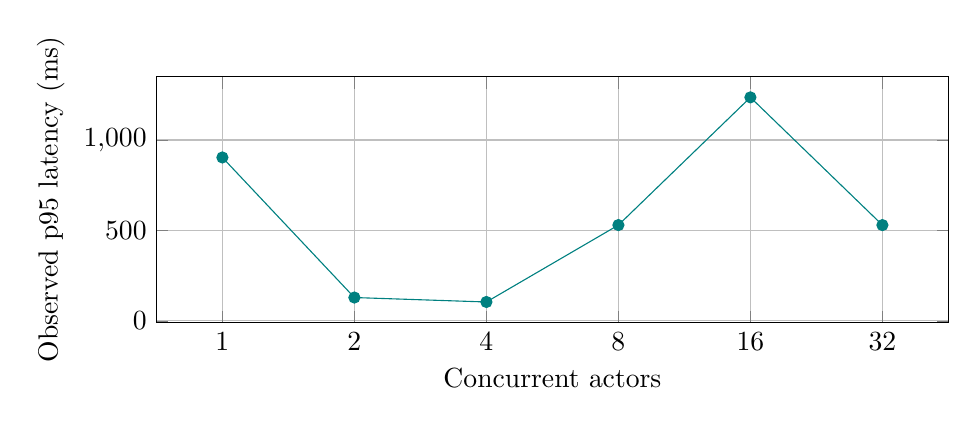
\begin{tikzpicture}
\begin{axis}[width=.96\columnwidth,height=4.7cm,xmode=log,log basis x=2,xtick={1,2,4,8,16,32},xticklabels={1,2,4,8,16,32},xlabel={Concurrent actors},ylabel={Observed p95 latency (ms)},grid=major]
\addplot[teal,mark=*] coordinates {(1,903.231) (2,129.245) (4,104.657) (8,529.672) (16,1235.35) (32,529.567)};
\end{axis}\end{tikzpicture}
\caption{Durable shared-budget races across separate OS processes; empirical p95 latency across recorded attempts at each population. Rejected requests and lock contention are included; setup is excluded.}\label{fig:v2latency}\end{figure}


\subsection{Safety and availability under CPU contention}
Repeated shared-budget races allow only one eight-unit effect against an
eight-unit shared capacity. Increasing actor count does not increase the
admitted charge. The latency figure retains the actor population, host, and
sample scope. It reports observed operation latency, including database
contention; it is not an estimate of inference latency or a hardware-independent
service-level guarantee.

In the scripted controller control, no enforcement and stateless per-call
checking both permit the individually valid requests to exceed the shared budget
when there is more than one actor. Durable enforcement with and without fencing
conserves it. That control does not separate the two durable controllers on
ordinary budget contention. Their difference is instead exposed by the
revocation fault controls: old accepted work can complete after admission
withdrawal, while a sink barrier rules out later old-authority effects after its
acknowledgment.

The delayed-fence result records a service cost rather than pretending that
withdrawal is instantaneous. With a 200-millisecond in-progress transaction,
the fence waits behind the sink writer. Its observed acknowledgment delay and
unavailable charge are included in the generated summary. The earlier effect is
already committed by acknowledgment; subsequent retries leave the independent
effect log unchanged. In separate cancellation controls, the charge becomes
available only after authoritative no-effect settlement. Neither outcome is
approximated by a timeout refund.

\subsection{Mutation witnesses}
All ten individual omissions and all 45 pairs have a searched witness. The
search records \VTwoTraces{} distinct traces in its declared subsequence
language. Conjunction and binding omissions allow wrongly authorized effects;
durability and timeout-quarantine omissions permit aggregate overspend after
recovery or late completion; omitting fencing permits an old effect after the
declared barrier. Deduplication failure can also cause repeated effects even
without a new broker reservation.

Many pairwise witnesses reuse the shorter witness for a single omitted
mechanism. We report the omission sets and their shortest searched witnesses,
not a count of newly discovered interactions or globally minimal attack
strategies. The complete model's lack of harm is confined to the same finite
language. Its positive task control makes reject-all behavior visible but does
not elevate that bounded search into a universal theorem.

\subsection{Benchmark controls and model feasibility}
The twelve declared AgentDojo tasks execute their native ground-truth calls
through upstream Progent's exact-policy checks, and all twelve pass the native
utility positive control in this run. Native attack graders also run on those
post-states, with their outputs retained. No import or integration error is
converted into a security failure. These results establish a runnable subset
and a working upstream policy-checking reference. They do not constitute the
planned model-generated policy or adaptive-attack comparison.

The checked Linux hosts have active GPU workloads. The local host and two
remote Linux aliases therefore fail the idle-resource precondition. A fourth
alias resolves to a differently named Darwin machine and fails the required
identity/architecture check. No GPU is allocated and no existing process is
preempted. The release records zero model GPU seconds, no chosen campaign
sample, and no holdout outcomes. Development timing cannot justify selecting
32, 64, or 128 campaigns without a usable model resource.

Consequently, the learned-review controller has no measured outcomes and the
five-way model comparison remains unrun. There is no checkpoint-specific
attack rate, confidence interval, or noninferiority conclusion. The artifact's
scientific claim is narrowed to executable policy verification and evaluated
local protocol behavior. A GPU validation of the managed inference runner and frozen
campaign run would be needed to support the intended model-facing usefulness
claim. Favorable CPU controls cannot fill that evidence gap.
